\documentclass[12pt]{article}
\usepackage{fontspec}
\defaultfontfeatures{Scale=MatchLowercase,Mapping=tex-text}
\setmainfont{Minion Pro}
\setsansfont{Myriad Pro}
\setmonofont{Lucida Sans Typewriter}
\usepackage{geometry}
\geometry{paperwidth=210mm,paperheight=297mm,top=20mm,left=25mm,right=25mm,bottom=30mm}
\usepackage[colorlinks]{hyperref}
\usepackage{graphicx}
\usepackage[magyar]{babel}
\frenchspacing
\sloppy

\newenvironment{code}{%
  \begin{list}{}{\raggedright\normalfont\ttfamily}\item[]}
  {\end{list}
}


\begin{document}

\title{Huhyphn -- magyar elválasztásiminta-gyűjtemény}

\author{Nagy Bence}

\maketitle

\begin{abstract}
A Huhyphn elválasztásiminta-gyűjtemény létrehozásának célja az élő
magyar nyelv szavainak hibátlan elválasztása szabad szoftveres környezetben.
A mintagyűjtemény a \TeX{}-ben és valamennyi a LibHnj programkönyvtárat
használó alkalmazásban -- a legjelentősebbek az OpenOffice.org és
a Scribus -- teszi lehetővé az algoritmus által megszabott keretek
közötti magyar nyelvű elválasztást.
\end{abstract}


\section{Áttekintés}

\subsection{Miért kell elválasztani?}

A klasszikus könyvművészet a szöveget mindig téglalap alakú szedéstükörbe
helyezte el. A nyelv szavai egy általános szövegben azonban sohasem
követik egymást olyan sorrendben, hogy egymás mellé helyezve egyenlő
hosszúságú sorokat alkossanak. A betűk szerkezeti felépítése, a betűk
egymásközti távolsága és a szavak közti távolság nemcsak esztétikai
kérdés, hanem az olvashatóság szempontjából is fontos.

Amikor \textsc{Johannes Gutenberg} a híres negyvenkét soros Bibliát
készítette, egységesen keskeny szóközöket alkalmazott. A sorkizárást
különböző szélességű betűk metszésével, ligatúrák és abbreviatúrák
alkalmazásával érte le. Noha a latin nyelv betűi és írásjelei mintegy
60 jelet tesznek ki, Gutenberg 290 különböző jelet metszett. A mai
napig esztétikai mintaképül szolgál.

Követője, \textsc{Peter Schöffer} vezette be a manapság is leggyakrabban
használt eljárást, a szóközök méretének változtatását. A szöveg szóközeinek
növelése vagy csökkentése révén lehet elérni az egyforma hosszúságú
sorokat. Esztétikai és olvasáspszichológiai okokból azonban nem szabad
eltérni nagymértékben az alapszóköz méretétől. Ez abban az esetben
valósítható meg jól, ha egy sorban minél több szóköz van, így az egyes
sorhosszkülönbségeket szétosztva, azok kisebb mértékben növelik vagy
csökkentik a szóközök méretét. Nemkívánatos az a jelenség, amikor
az egyes szóközök mérete olyan nagymértékben nő, hogy azok akár a
sorok közti távolságot is meghaladják.

Mivel a magyar nyelv agglutináló, vagyis a szótőhöz hozzáilleszti
a toldalékokat, a szövegben a hosszú szavak igen gyakoriak, így az
elválasztások alkalmazása nélkülözhetetlen, ha igényes szedés kialakítása
a célunk. Ennek jelentősége nyomtatott dokumentumok esetén van, az
interneten legelterjedtebb HTML-formátumú weboldalak nem tartalmaznak
elválasztást, és alapesetben nem sorkizárt szövegeket jelenítenek
meg.


\subsection{Az elválasztás jelentősége}

Amíg a \TeX{}-rendszer főleg tudományos körökben használt eszköz maradt
fejlesztésének évei alatt, a Liang-féle elválasztó algoritmus problémái
csak kevés embert érintettek. Mivel a \TeX{} nyílt rendszer, ezért
bárki készíthet hozzá kiegészítéseket, javításokat, így korábban a
szakértő felhasználók is orvosolni tudták gondjaikat, és elmondhatjuk,
hogy a \TeX{} szellemiségébe beleillik ez a fajta felhasználói változtatás.

Az OpenOffice.org általános célú irodai programcsomag, amelybe szintén
ezt az elválasztó algoritmust építették be, azonban ez a rendszer
már a szélesebb közönséget célozza meg. A program a ,,középiskolás
fokon'' oktatott számítástechnikai ismeretekkel is egyszerűen használható,
ezért elterjedése nem lehet kétséges. Mivel szabadon terjeszthető,
ezért a Linux operációs rendszer elsőszámú irodai programcsomagjává
vált, és része a legtöbb disztribúciónak -- aki egy modern Linux disztribúciót
telepít, az előbb-utóbb találkozik a programmal. Az asztali gépen
Linuxot használók száma még csekély a Microsoft Windows felhasználóihoz
képest, de valószínűleg ez utóbbi platformon is gyorsan fog nőni a
programot használók száma, nem beszélve a többi operációs rendszerről,
amelyen elérhető.

Az OpenOffice.org-ba épített LibHnj programkönyvtárat \textsc{Raph
Levien} írta 1998-ban, ennek a magas szintű elválasztás és sorkiegyenlítés
a feladata. Forráskódja szintén szabadon felhasználható, ezért várható,
hogy újabb programokba is be fogják építeni.

Az egyik ilyen ismert alkalmazás, a Scribus tördelőprogram, melynek
2003. júliusában jelent meg az 1.0-s verziója, és jelenleg úttörőnek
mondható a Linuxos DTP területén. Felhasználóinak száma minden bizonnyal
alacsonyabb az OpenOffice.org\emph{-}énál, viszont ezen a területen
nagyobb a jó elválasztás jelentősége.

Magyar nyelvű szövegek szedésének egyik sarkalatos pontja a helyes
elválasztás. A helytelen elválasztás helyesírási hiba, az elválasztások
kihagyása azonban a sorkizárt szövegben okozhatja a fent említett
szóközanomáliát. Nyelvünknek speciális elválasztási kívánalmai is
vannak. A nyelvben több egyszerűsítve kettőzött hosszú mássalhangzó
van, melyeket nem egyszerűen csak kettéválasztunk, hanem bizonyos
betűk a két elválasztott részben megismétlődnek. Hogy érthetőbbé tegyem:
az \emph{asszony} szó az \emph{asz-} és a \emph{szony} tagokra választandó
szét, erre azonban a \TeX{} beépített algoritmusa nem alkalmas. Mivel
az ilyen betűk előtt is és után is egy-egy magánhangzó van, ha nem
tudjuk elválasztani a szót, úgy egy legkevesebb öt betűből álló láncot
kapunk, mely gondot okozhat az egyenletes szóközök terén, ha a szó
pont a sor végére esik.

A \TeX{} egész bekezdést vizsgáló sortörő algoritmusa annyira kifinomult,
hogy optimális használatához a forrást a lehető legjobban kell előkészíteni.


\subsection{A magyar nyelv elválasztási szabályai}

A magyar nyelvnek egyszerűek az elválasztási szabályai: a szavakat
szótagokra kell bontani, és az a szótaghatárok mentén elválasztható.
A szótagoló elválasztás nem alkalmazható összetett szavak esetén maradéktalanul,
itt a szóösszetétel határára kell esnie az elválasztásnak. A szabály
idegen szavak esetében a kiejtés szerinti szótagolást részesíti előnyben,
ezért sok idegen szó számít csak egy szótagosnak és nem elválaszthatónak,
még ha az eredeti alakban vagy annak átvett változatában több magánhangzó
is szerepel.

A fenti két szabály ütközik, és ennek következtében a magyar elválasztási
szabályok nem adnak egyértelmű utasítást arra az esetre, ha idegen
eredetű szavak szerepelnek a szóösszetételekben. Ilyenkor \emph{A
magyar helyesírás szabályai}-ban leírtak szerint a meghatározatlan
,,átlagos magyar nyelvérzéknek'' kell döntenie, hogy elfogadja-e valamely
összetevőt a magyarban is élő alaknak vagy pedig a szóösszetételtől
függetlenül szótagolás szerint kell elválasztani.

A szótagolás szerinti történő elválasztás módszerét a szabályzat 226.
paragrafusa tartalmazza. Rövid algoritmusa a következő: minden magánhangzó
új szótagot jelöl, és a magánhangzók előtt szereplő mássalhangzók
közül mindig az utolsót kell átvinni a következő sorba, és itt a tényleges
másalhangzót kell érteni, többjegyű esetén valamennyi betűjének az
új sorba kell átkerülnie.

Erre az algoritmusra könnyű programot írni, ez azonban csak a magyar
nyelvre lesz használható, a HiOn is eszerint működik és a \TeX{} magyar
elválasztási mintáinak 3.12-es verziójáig az ezt megvalósító mintahalmazzal
rendelkezett. Az összetett szavak elválasztásának problémáját mindkettő
a szó kivételszótárba, illetve a minták közé történő közvetlen felvételével
oldotta meg. Ennek hátránya nyilvánvaló: a szóösszetételek száma hatalmas,
és ebben az esetben a hibásan elválasztott összetett szavakkal folyamatosan
kell bővíteni a szótárakat.


\subsection{A \TeX{} módszere}

A \TeX{}-rendszerbe \textsc{Frank M. Liang} elválasztási algoritmusát
építették be, amely előre megadott minták alapján határozza meg az
elválasztási helyeket, és így bizonyos megszorításokkal valamennyi
latin betűs nyelvre alkalmazható.

Liang 1980 és 1982 között dolgozta ki, és \emph{Word hy-phen-a-tion
by computer} című doktori értekezésében 1983-ban publikálta a számítógéppel
történő elválasztás egy módszerét, amelyet a \TeX{}-rendszerbe is
beépítettek. A Liang-algoritmus gyorsan működik, és valamennyi olyan
elválasztási helyet bejelöl, amelyet az elválasztási mintái között
eltárolunk. Az algoritmust megvalósító kód igen egyszerű és kevés
memóriát igényel, ez az állítás pedig tizenöt évvel kitalálása után
hatványozottan igaz.

A \TeX{} a következőképpen választ el. Ha megkap egy szót, először
megnézni a kivételszótárat, hogy nincs-e definiálva benne ennek a
szónak a különleges elválasztása. Amennyiben nem szerepel benne, úgy
a Liang-algoritmussal választja el.

Az angol \texttt{hyphenation} szó elválasztásán keresztül mutatom
be az algoritmus működését, Knuth maga is ezt a példát hozza fel,
és \textsc{Fricz Cremer}, a \emph{The \TeX{}book} németre fordítója,
is ragaszkodott ehhez.

Az algoritmus a szót először kiegészíti két ponttal: \texttt{.hyphenation.},
majd pedig felbontja egyre növekvő hosszúságú szakaszokra. A pontok
a szó elejét és végét jelentik, ennek fontos szerepe van, némelyik
elválasztási minta konkrétan csak szó eleji vagy végi helyzetben ad
helyes elválasztást.

Az így kapott egybetűs szakaszok:

\begin{code}
.~h~y~p~h~e~n~a~t~i~o~n~.
\end{code}

a kétbetűsek:

\begin{code}
.h~hy~yp~ph~he~en~na~at~ti~io~on~n.
\end{code}

hárombetűsek:

\begin{code}
.hy~hyp~ype~pen~ena~nat~ati~tio~ion~on.
\end{code}

és így tovább.

Az így létrejött \texttt{k} hosszúságú szakaszokhoz \texttt{k+1} számot
társít, melyek az egyes betűk előtt fogják jelölni az elválasztási
helyeket. A \texttt{hen} szakaszhoz négy szám kerül majd, melyet a
következképpen lehet szemléltetni:

\begin{code}
0h0e2n0
\end{code}

A 2-es számjegy az \texttt{e} betű utáni lehetséges elválasztás információját
tartalmazza.

Az elválasztás folyamata a továbbiakban úgy zajlik, hogy a program
az előre eltárolt elválasztási mintákból megkeresi azokat, amelyek
megegyeznek a szó szétbontott szakaszaival. A \texttt{hyphenation}
szóra az angol nyelvi szótárból a következőeket találja meg:

\begin{code}
0h0y3p0h0

0h0e2n0

0h0e0n0a4

0h0e0n5a0t0

1n0a0

0n2a0t0

1t0i0i0

2i0o0

0o2n0
\end{code}

Az elválasztás utolsó lépése az, hogy az egyes betűk közé jutó értékek
közül mindig a legnagyobbat választja ki, majd a szavunkba illeszti
azokat. A szó végül így fog kinézni:

\begin{code}
0h0y3p0h0e2n5a4t2i0o2n0
\end{code}

Ahol a szóban páratlan szám található, ott elválasztható a szó, ahol
páros vagy nulla, ott nem engedélyezett az elválasztás. A hyphenation
szó tehát elválasztva: \texttt{hy-phen-ation}.

Ha összehasonlítjuk Liang doktori értekezésének címét és a végeredményt,
lehet látni, hogy ez utóbbiban eggyel kevesebb elválasztási hely lett
bejelölve, maga Knuth azt írja, hogy az elválasztási algoritmus az
elválasztási helyek döntő többségét megtalálja. Megfelelően kialakított
mintafájl esetén azonban valamennyi elválasztási helyet megkapjuk.


\subsubsection{A módszer hiányosságai}

Az algoritmus egyik nagy hiányossága, mely minket különösképpen érint,
hogy nem képes az egyszerűsítve kettőzött hosszú mássalhangzókat elválasztani.

A \TeX{} elválasztórendszerének másik hiányossága, hogy nem választja
el azokat a szavakat, amelyekben kötőjel van. A 6--3-as szabály miatt
a hosszú szóösszetételeket kötőjellel kell írni, de földrajzi nevekben
is sokszor fordul elő ez az írásmód.

Erre a problémára megoldást jelent \textsc{Bernd Raichle} \texttt{hypht1.tex}
nevű fájlja, azonban ehhez mélyebben nyúl bele a \TeX{} elválasztórendszerébe.
A \texttt{\textbackslash{}hyphenation} makróval lehet elválasztásokat
megadni, amelynek kötőjellel elválasztott szavakat kell megadni. Kötőjeles
alak esetén a kötőjel elé egy egyenlőségejelet kell írni: \texttt{\textbackslash{}hyphenation\{Er-zsé-bet=-híd\}}.

A \LaTeX{} Babel csomagjához készült stílusfájlban sikerült megoldani
az egyszerűsítve kettőzött hosszú mássalhangzók elválasztásának problémáját,
azonban az csak jelentős többletmunka árán kelthető életre. A trükk
lényege, hogy ezeket a karaktersorozatokat külön meg kell jelölni
egy fordított aposztróffal: pl. \texttt{lo`ccsan}, \texttt{frö`ccsen}.


\section{A szótárfejlesztés}


\subsection{A régebbi modulok által felvetett kérdések}

A Huhyph 3.12 és Huhyph 4.0 esetén alkalmazott módszerek akármelyikét
vizsgálva jelentős nehézséggel kerülünk szembe.

A kézzel szerkesztett fonetikai bázisra épülő változatnál rengeteg
szót kell megvizsgálni és a rájuk alkalmazható mintákat megtalálni.
Az új minták felvétele esetén meg kell vizsgálni a régebbieket, hogy
azok módosításával elérhető-e a kívánt eredmény, vagy az új minta
felvétele esetén találkozunk-e olyan szóval, amelyiket eddig helyesen
választott el, de az új minta felvételével már hibásan.

A Huhyph 4.0 módszerével készített kollekció esetén pedig akkor érhetünk
el optimális eredményt, ha egy szóhóz valamennyi képzett alakjának
elkészítjük az elválasztott formáját, és felvesszük a szótárba. A
Huhyph 4.0 szókészlete nem haladja meg a 70000-es méretet, a mintagenerálás
folyamata azonban a dokumentációja szerint egy 1 GHz-es Pentium IV-es
számítógépen majdnem nyolc percet vesz igénybe. Amennyiben minden
szónak további változatait képezzük, úgy a művelethez szükséges idő
nagyságrendekkel nőhet, és akár órákig is tarthat. Nem lehetünk azonban
biztosak ekkor sem abban, hogy a szótárból hiányzó szavak megfelelően
választódnak el, csak reménykedhetünk, hogy a szótár növekedésével
a fonetikai szabályok és a növekvő számú azonos kivételek átlépik
azt a kritikus tömeget, hogy érvényesüljenek a nem felvett szavakra
is.


\subsection{A PatGen}

A PatGen kiválóan használható alkalmazás, hogyha meg tudjuk kerülni
a használatából származó hátrányait. A fenti problémák alapján két
elvárásnak kell megfelelni:

\begin{itemize}
\item A generált minták tartalmazzák teljes egészében a fonetikai szabályokat,
hogy a szótárban nem szereplő szótagok esetén is érvényesüljenek.
\item A generált minták ne befolyásolják a fonetikai szabályok szerint választandó
szavak elválasztását.
\end{itemize}
Az első elvárást egyszerű teljesíteni, a PatGen-t előre elkészített
mintákkal kell meghívni, amelyek tartalmazzák a szótagolás szerinti
elválasztás szabályait.

A második elvárás teljesítése a nehezebb, ugyanis itt a PatGen működése
okozza a problémát. A program ugyanis a bemeneti szótárt alapul véve
határozza meg az összetétel szerint elválasztandó szavak esetében
a szükséges alkalmazandó mintát. Mivel optimális megoldásra törekszik,
ezért ez a minta a lehető legrövidebb lesz, és így könnyen előfordulhat
az, hogy egy szótárban nem szereplő, a fonetikai szabályokkal elválasztható
szónál hibás elválasztást fogunk kapni.

A PatGen megfelelő paraméterezésével érhetjük el, hogy ne törekedjen
optimális eredmény generálására, de ebben az esetben is a bemeneti
szótár duzzasztására van szükség. Nem agglutináló nyelvek esetén bőven
elég lenne a szó felvétele a szótárba, de a magyarban minél több toldalékolt
alakot fel kell venni. Erre egy módszer, ha könyvek szavait a Hunspell-en
keresztül átszűrjük. Ez a helyesírás-ellenőrző meg tudja mondani egy
szóról, hogy az valamely szótőnek a toldalékolt alakja-e. Ha ismerjük
a szótő elválasztását, akkor a toldalékolt alak elválasztását is meghatározhatjuk,
mivel a toldalékok minden esetben a fonetikai szabályok szerint választandók
el. A szótár növekedése ebben az esetben nem lesz annyira drasztikus,
minta egy algoritmussal valamennyi létező toldalékolt alakot felvennénk,
ugyanis így csak a ténylegesen használt formák kerülnek a szótárba.

A PatGen alkalmazásával elkerülhető, hogy a \TeX{} kivételszótárát
kelljen használni az ismeretlen vagy hibás elválasztású szavak esetén,
elég a szót felvenni a program bemeneti szótárába, és az új mintafájl
már megfelelően fogja kezelni ezt a szót is.

A szótár gyarapodásával együtt jár a feldolgozási idő növekedése,
de ezt az árat meg kell fizetnünk.


\subsection{A Szószablya}

A Szószablya projekt (\url{http://www.szoszablya.hu/}) a magyar web
feldolgozásával olyan szóanyagot állított össze, amely a ma beszélt
magyar nyelv szókészletét nagy mértékben lefedi. A teljes szóanyagból
a nagy gyakorisággal előfordulóakat kiválogatva és a Hunspell helyesírás-ellenőrzőn
átszűrve olyan szótárat kapunk, amely ideális lehet az elválasztási
mintagyűjtemény bemeneteként.


\section{Fejlesztőkörnyezet}


\subsection{Források}


\subsubsection{Patgen}

A minták generálását a te\TeX{} disztribúció patgen alkalmazása végzi.
A \texttt{magyar.tra}, a \texttt{patgen.in} és a \texttt{base.pat}
fájlok a program működéséhez szükséges paramétereket tartalmazzák.
A patgen.patch alkalmazása a nagy mennyiségű adat feldolgozásához
szükséges, jelenleg nem ismert, hogy ilyen paraméterek mellett mekkora
bemeneti szótár feldolgozására képes, a mintegy 2700000 szavas állomány
esetén sikerrel használható.


\subsubsection{Substrings.pl}

Az OpenOffice.org a módosított algoritmusú LibHnj-t használja, ehhez
a csomagban lévő \texttt{substrings.pl} használatával a kész minták
átalakítására van szükség.


\subsubsection{A szótár}

A bemeneti szótár mintegy 45 MB méretű, a szótár magját képező szógyűjteményt
a \texttt{web2.2-mostfrequent-hungarian-words.txt.gz} fájl tartalmazza,
ezt a Szószablya projekt weboldaláról lehet letölteni. A majdnem teljes
bemeneti szótár előállításához a \texttt{test.rb} program módosításával
juthatunk, ha azt csővezetékbe kötve futtatjuk a fenti fájlon.


\subsection{Működés}

A folyamat a \texttt{Makefile}-on keresztül a \texttt{make} parancs
kiadásával történik. A \texttt{patgen} formátumfüggetlen mintagyűjteményt
hoz létre, melynek felhasználásával az \texttt{eruby} program (ezt
külön kell telepíteni) a \texttt{.tmpl} végű sablonfájlokból elkészíti
a mintagyűjtemény különböző változatait.


\section{Telepítés}


\subsection{Telepítés \TeX{} alá}

A \TeX{}-rendszerhez rendelkezésre álló mintagyűjtemény a \texttt{.tex}
nevű fájlban található. A fájlban található karakterek az EC-, T1-
vagy más néven Cork-kódolás szerint szerepelnek. Ez a szokásos magyar
nyelvű \LaTeX{} használat mellett eredményezi a megfelelő működést.
A fájlt a texmf-fa \texttt{/tex/generic/hyphen} könyvtárába kell másolni,
majd a \texttt{mktexlsr} programmal frissíteni a fájlnyilvántartást.

A fájl megfelelő helyre másolása és a konfigurációs fájlok szükséges
módosítása után szükség van a formátumfájlok legenerálására, mivel
a szótárak feldolgozása nem futásidőben történik. A te\TeX{}-rendszeren
a beállítások végrehajthatóak a \texttt{texconfig} programmal, amely
a különböző makrócsomagoknál teszi lehetővé az eltérő beállítás használatát,
és gondoskodik a formátumfájlok elkészítéséről is. Az alábbiakban
a kézzel történő beállítások találhatóak.


\subsubsection{\LaTeX{}}

A \LaTeX{} makrócsomag esetén a betöltendő elválasztási minták a \texttt{language.dat}
fájlban találhatóak. Ennek szokásos helye a texmf-fa

\begin{code}
/tex/generic/config
\end{code}
könyvtár. Szerepelnie kell benne egy

\begin{code}
magyar~huhyph.tex
\end{code}
tartalmú sornak, esetleg százalékjellel az elején. Ezt a sort tegyük
megjegyzésbe, és egy másik sorba írjuk a következőt:

\begin{code}
magyar~huhyphn.tex
\end{code}
A formátumfájl legenerálásakor már a Huhyphn elválasztási mintái épülnek
be.


\subsection{Telepítés OpenOffice.org alá}

Az \emph{OpenOffice.org} irodai programcsomaghoz használható elválasztási
mintafájl a \texttt{hyph\_hu.dic} nevet viseli. Ezt a következő könyvtárba
másolva írjuk felül az eredeti változatot (a könyvtár disztribúciótól
függően változhat):

\begin{code}
/usr/lib/OpenOffice.org/share/dict/ooo/
\end{code}
A program ezek után már a \emph{Huhyphn} elválasztási mintáit használja.

\begin{figure}
\begin{centering}
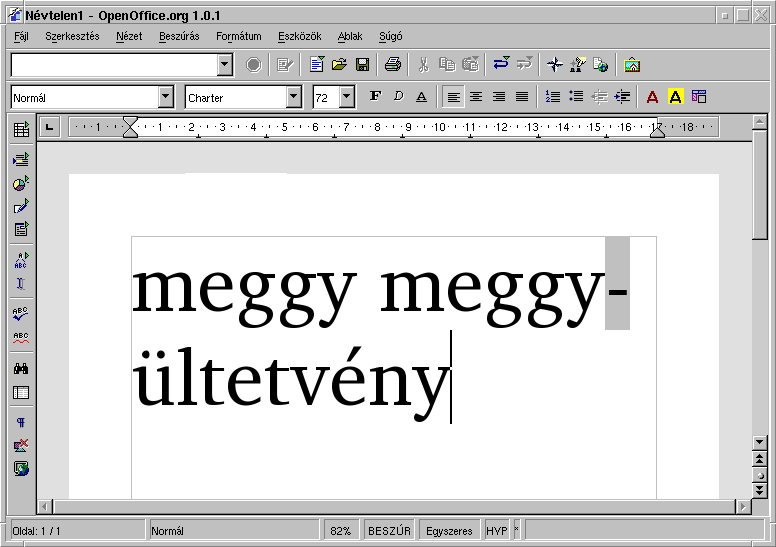
\includegraphics[scale=0.5]{oo1}
\end{centering}
\caption{Az \emph{OpenOffice.org} ablakában immár a helyes elválasztás.}
\end{figure}


\begin{figure}
\begin{centering}
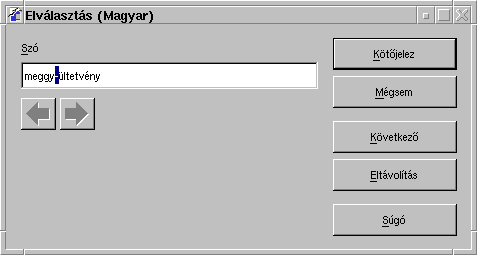
\includegraphics[scale=0.5]{oo2}
\end{centering}
\caption{Az elválasztás engedélyezésének ablaka.}
\end{figure}


\subsection{Telepítés Scribus alá}

A \emph{Scribus} az elválasztási mintákat a

\begin{code}
/usr/lib/scribus/dicts/
\end{code}

könyvtárban tárolja, ide kell másolni a \texttt{hyph\_hu.dic} fájlt
(az 1.1-es verzió nem engedi szimlink használatát).


\section{Elérhetőség}

A \url{http://www.tipogral.hu/} oldalon érhetőek el a projekt keretében
létrehozott elválasztómodulok és programok, melyeket a GPL
feltételei szerint lehet felhasználni.

\end{document}

